%%%%%%%%%%%%%%%%%%%%%%%%%%%%%%%%%%%%%%
% Numerical Linear Algebra class 2022 
% Solutions to Sheet 8
%%%%%%%%%%%%%%%%%%%%%%%%%%%%%%%%%%%%%%

\begin{SolutionSheet}[\ref{sheet8}]

  \begin{Solution}
    \begin{enumerate}[(a)]
    \item Sample calculation of LU factorization in
      \lstinline{./programs/lu.py}. Sparsity patterns in figure below.

      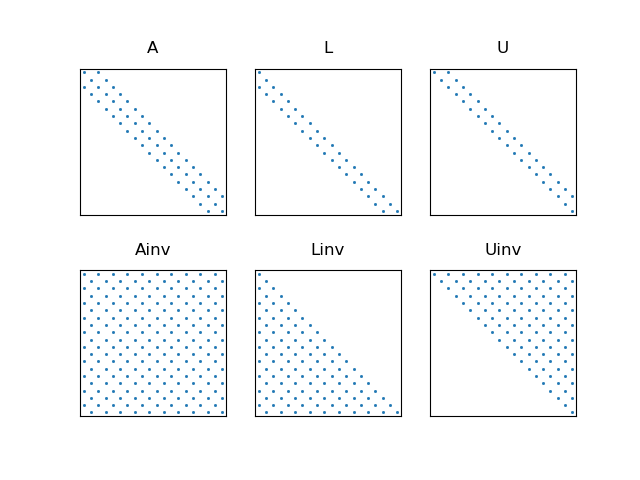
\includegraphics[width=0.8\textwidth]{figures/lu-decomposition-of-sparse-matrix}
    \item The width of the zero diagonals gets transported to the
       matrices of the LU factorization

      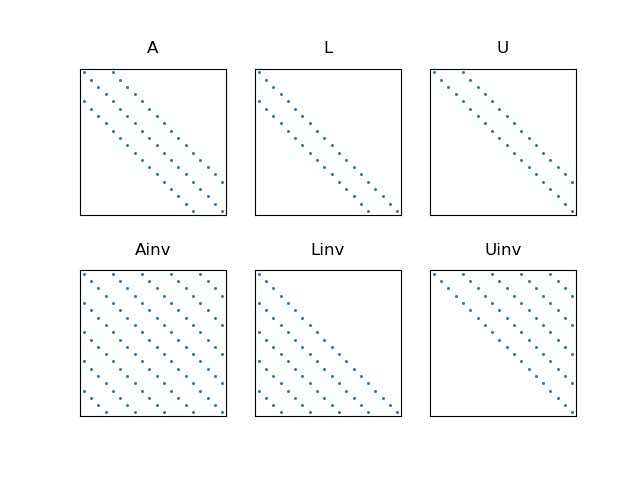
\includegraphics[width=0.8\textwidth]{figures/lu-decomposition-of-sparse-matrix-off4}
    \item The inverse is dense up to the zero diagonals that get
      scattered over the whole inverse
    \end{enumerate}

    
  \end{Solution}

  \begin{Solution}[{\cite[P-5.1 b]{Saad00}}]
    We start with some preliminaries before we prove the statement.

    Hint 1:
    \begin{gather*}
      \scal(\mata\vd^{(k+1)},\vd^{(k+1)})
      =\scal(\mata\vd^{(k)},\vd^{(k)})
      -\frac{\scal(\vr^{(k)},\ve_i)^2}{a_{ii}}
    \end{gather*}

    Hint 2:
    \begin{gather*}
      \abs{\ve_i^T \vr^{(k)}} \geq n^{-\nfrac12}\norm{\vr^{(k)}}_2
    \end{gather*}

    1. Since $\ve_i\in K=L$, it holds the Galerkin-orthogonality
    \begin{align*}
      \scal(\vr^{(k)}-\mata \ve_i,\ve_i) = 0,
    \end{align*}
    which leads to the equalities
    \begin{align*}
      a_{ii}
      = \ve_i^T\mata \ve_i,
      = \scal(\mata \ve_i,\ve_i)
      = \scal(\vr^{(k)},\ve_i)
      = \abs{\ve_i^T\vr^{(k)}}
      = \norm{\vr^{(k)}}_{\infty}
    \end{align*}
    meaning that $a_{ii}$ is not only an element of the diagonal of
    $\mata$, but also the maximal value of the residual vector, since
    $i$ has been chosen that way.

    2. By 1. we have
    \begin{align*}
      a_{ii} = \abs{\vr^{(k)}_i} = \abs{e_i^T \vr^{(k)}}.
    \end{align*}
    Thus, with the help of Hint 2,
    \begin{align*}
      \frac{\scal(\vr^{(k)},\ve_i)^2}{a_{ii}}
      = \frac{\abs{\ve_i^T\vr^{(k)}}^4}{\abs{\ve_i^T\vr^{(k)}}}
      = \abs{\ve_i^T\vr^{(k)}}^3
      = a_{ii} \abs{\ve_i^T\vr^{(k)}}^2
      \geq \frac1n a_{ii}\norm{\vr^{(k)}}_2
    \end{align*}

    3. Next, we have by definition
    \begin{align*}
      \mata\vd^{(k)}
      = \mata\left(\mata^{-1}\vb-\vx^{(k)}\right)
      = \vb-\mata\vx^{(k)}
      = \vr^{(k)},
    \end{align*}
    and
    \begin{align*}
      \vd{(k)}
      = \mata^{-1}\vb-\vx^{(k)}
      = \mata^{-1}\left(\vb-\mata\vx^{(k)} \right)
      = \mata^{-1} \vr^{(k)},
    \end{align*}
    implying
    \begin{align*}
      \frac{\scal(\mata\vd^{(k)},\vd^{(k)})}{\norm{\vr^{(k)}}^2}
      = \frac{\scal(\mata^{-1}\vr^{(k)},\vr^{(k)})}{\scal(\vr^{(k)},\vr^{(k)})}
      = R_{\mata^{-1}}(\vr^{(k)})
      \leq \lambda_{\max}(\mata^{-1})
      = \frac1{\lambda_{\min}},
    \end{align*}
    where
    $R_{\mata^{-1}}(\vx)=\frac{\scal(\mata^{-1}\vx,\vx)}{\scal(\vx,\vx)}$
    is the Rayleigh-quotient

    \begin{todo}
      4. We assume that
      \begin{align*}
        a_{ii} \geq \frac1{\lambda_{\max}}.
      \end{align*}
    \end{todo}

    \textbf{Proof:} With the help of Hint 1 and the forgoing
    statements we get
    \begin{align*}
      \norm{\vd^{(k+1)}}_{\mata}^2
      = \scal(\mata\vd^{(k+1)},\vd^{(k+1)})
      &\stackrel{\text{Hint 1}}{=}
        \scal(\mata\vd^{(k)},\vd^{(k)})
        - \frac{\scal(\vr^{(k)},\ve_i)^2}{a_{ii}}
      \\
      &=
        \left( 1 - \frac{\scal(\vr^{(k)},\ve_i)^2}{a_{ii}}
              \frac1{\scal(\mata\vd^{(k)},\vd^{(k)})} \right)
        \norm{\vd^{(k)}}_{\mata}^2
      \\
      &\stackrel{2.}{\leq}
        \left( 1 - \frac{a_{ii}\norm{\vr^{(k)}}^2}{n}
              \frac{1}{\scal(\mata\vd^{(k)},\vd^{(k)})} \right)
        \norm{\vd^{(k)}}_{\mata}^2
      \\
      &\stackrel{3.+4.}{\leq}
        \left( 1 - \frac{1}{n}
              \frac{\lambda_{\min}}{\lambda_{\max}} \right)
        \norm{\vd^{(k)}}_{\mata}^2
      \\
      &=
        \left( 1 - \frac{1}{n\cond(\mata)} \right)
        \norm{\vd^{(k)}}_{\mata}^2
    \end{align*}
    
  \end{Solution}

  \begin{Solution}
  \end{Solution}

  \begin{Solution}[Programming]
    C++ sample code \lstinline{./programs/steepest-decent.cc} without
    assembling the system matrix.

    Convergence rate (Definition 2.2.18 in lecture notes).  As can be
    seen in the plot, the convergence of the steepest decent method is
    sublinear.
    
    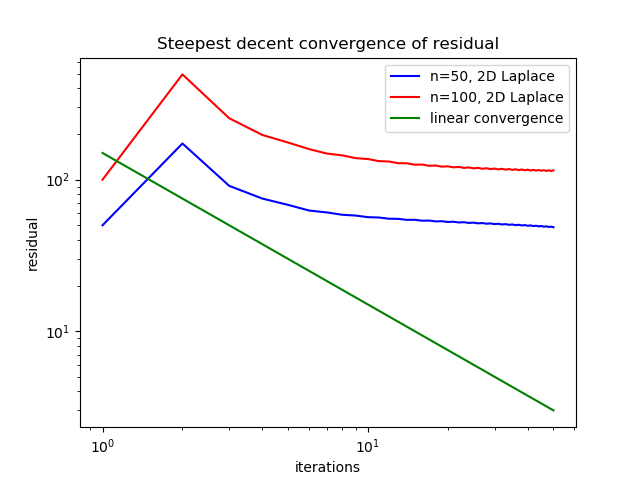
\includegraphics[width=\textwidth]{figures/laplace-steepest-decent}
  \end{Solution}

\end{SolutionSheet}


%%% Local Variables: 
%%% mode: latex
%%% TeX-master: "main"
%%% End: 
